\documentclass[floatfix,aps,prd,amsmath,amssymb]{revtex4}

\usepackage{epsfig}
\usepackage{color}
\usepackage{graphicx}
\usepackage{float}
\usepackage{listing} %listings
\usepackage{braket}
\usepackage{mathtools}

\begin{document}
% cite:
% SCPV1 ! INTRO (CP3 Seminar)
% SCPV2 SUSY SCPV SO(10)
% SCPV3 Szekeres
% SCPV4 GUT Algebra Baez
% SCPV5 SCPV Group Conditions
% SCPV6 Local Gauge Invariance
% SCPV7 Apson Model
\section{Spontaneous Charge Parity Violation} 
A major motivation for creating models with new CPV mechanisms is to explain Baryon asymmetry. This is a huge research area, a simple search on arXiv.org reveals over $500$ papers. The most prevalent theories are based around Super-Symmetry (SUSY) and Spontaneous Charge Parity Violation (SCPV). 

Typically these models are created by looking for gauge symmetries which coincide with Lagrangians similar to the Standard Model, but with extra terms that may account for the preference of antimatter to decay into matter.  

SCPV is praised for its ``naturalness" in comparison to regular CPV\cite{SCPV1}. It supposes the possibility to have spontaneous CPV by the vacuum, as opposed to explicit CPV from the CKM matrices. That is, the vacuum is no longer invariant under CP. In a sense this is nice as it may not introduce as many new particles. Indeed, the Minimal SUSY Standard Model is not compatible with SCPV, and in general it is difficult to incorporate SCPV in SUSY models\cite{SCPV1}, but it has been done. For example in SUSY $\mathrm{SO}(10)$ \cite{SCPV2}.

There are two primary goals to this section. First, to elucidate the use of groups in physics, particularly particle physics. Second, to use this knowledge to understand various SCPV  models beyond the insufficient description given in this introduction.

\subsection{SCPV. Group Theory for Physics}
Some physicists take pride in never having learned group theory and still understanding its applications. This is not an unreasonable point of view, an engineer can launch a rocket without knowing real analysis. 

Undergraduate group theory modules quite commonly focus entirely on groups useful for pure mathematics. This is understandable as it is taught by the math department, but the picture of group theory young physicists may end up with is often quite different to its use in physics.


Part of the reasons groups can be so abstract is that they have very little structure. Even basic physics requires complicated structure. Simply changing coordinates in classical mechanics requires differential geometry, which requires analysis and topology. A \textbf{Group} is a set $G$ with a function $\cdot:G^2\rightarrow G$, having the following properties $\forall g,h,k \in G$
\begin{align*}
\begin{array}{l l l}
(\mathrm{GA}1) & g\cdot h \in G & \text{closure} \\
(\mathrm{GA}2) & \exists e\in G,\phantom{a} e\cdot g = g \cdot e = g \phantom{a}& \text{identity} \\
(\mathrm{GA}3) & \exists g^{-1}\in G, \phantom{a} g^{-1} \cdot g = g \cdot g^{-1} = e & \text{inverse} \\
(\mathrm{GA}4) & (g\cdot h)\cdot k = g\cdot(h \cdot k) & \text{associativity} \\
\end{array}
\end{align*}
Abstract definitions will be avoided in general. To understand this proceed with a useful example. Let $\mathrm{GL}(n,\mathbb{R})$ be the set of all $n\times n$ matrices with real coefficients and non-zero determinant. This forms a group under matrix multiplication.
\begin{itemize}
\item[(GA1)] The product of two $n\times n$ matrices is an $n \times n$ matrix, so it is closed.  
\item[(GA2)] The identity matrix $I$ satisfies $IM=MI=M$.
\item[(GA3)] Non-zero determinant matrices are invertible $M^{-1}M=MM^{-1}=I$.
\item[(GA4)] As real multiplication and addition are associative ($(1+2)+3=1+(2+3)$) Matrix multiplication inherits this property.
\end{itemize}
\textsc{Note:}
\begin{itemize}
\item The set of all real matrices would fail, as zero determinant matrices do not have inverses.
\item Associativity is usually trivial by the definition and not checked.
\end{itemize}
The purpose of this proof was to give some familiar meaning to the abstraction. Detailed proofs shall be avoided in favour of intuition. Note that already  a more powerful structure is present than a group, the field of real numbers, $(\mathbb{R},+,\times)$. This is essentially just two groups glued together, addition and multiplication.

Similarly, every vector space is a group under vector addition. With this it could be said that all of physics uses groups, however a secondary school student does not use differential geometry with Newton's laws. At this stage groups are still useless to the practical physicist.

A \textbf{transformation group} is a more useful idea. Let $X$ be a set, $\mathrm{Transf}(X)$ is the set of all one-to-one functions from $X$ to $X$. This is the set of all ways of rearranging $X$. In the context of a finite group $S=\{1,2,...,n\}$, $\mathrm{Transf}(S)$ is just the set of all permutations. 

If $3$-dimensional space was modelled by $\mathbb{R}^3$ the transformation group would not be useful, it would contain unnatural discontinuous functions that do not relate to intuition about space. What would be useful is:
\begin{center}
The transformations that preserve a property of a space form a group. It is known as the \textbf{invariance group} or the \textbf{symmetry group}.
\end{center}
 This is an extremely general and potent idea. It is also not difficult to prove, so it shall be after the following motivation.
 
Model space again as $\mathbb{R}^3$, transformations should preserve distance. Where Euclidean distance is defined by
\begin{align*}
d(\mathbf{x},\mathbf{y})\vcentcolon = \sqrt{(x_1-y_1)^2+(x_2-y_2)^2+(x_3-y_3)^2}
\end{align*}
 The desired transformation $\mathrm{R}$ has form such that $d(\mathrm{R}\mathbf{x},\mathrm{R}\mathbf{y}) = d(\mathbf{x},\mathbf{y})$. From intuition there are some obvious transformations $\mathrm{R}=I$, the identity matrix, or $\mathrm{R}\mathbf{x} = \mathbf{x}+\mathbf{a}$ a translation in space
\begin{align*}
d(\mathrm{R}\mathbf{x},\mathrm{R}\mathbf{y}) &= d(\mathbf{x}+\mathbf{a},\mathbf{y}+\mathbf{a}) \\
&= \sqrt{\sum_{i=1}^3((x_i+a_i)-(y_i+a_i))^2} \\
&= \sqrt{\sum_{i=1}^3(x_i+a_i-y_i-a_i)^2} \\
&= \sqrt{\sum_{i=1}^3(x_i-y_i)^2} \\
&= d(\mathbf{x},\mathbf{y})
\end{align*}
Now note
\begin{align*}
d(\mathbf{x},\mathbf{y})^2=(\mathbf{x}-\mathbf{y})\cdot(\mathbf{x}-\mathbf{y})
\end{align*}
Where $\cdot$ is the regular dot product. Calling $\Delta\mathbf{x}\vcentcolon =\mathbf{x}-\mathbf{y}$ and using serif font to signify matrix representation
\begin{align*}
\Delta\mathbf{x}\cdot\Delta\mathbf{x} &= \mathsf{\Delta x}^T \mathsf{\Delta x} \\
&= (\mathsf{x}-\mathsf{y})^T(\mathsf{x}-\mathsf{y})
\end{align*}
In other words dot product in an orthonormal basis is a row vector times a column vector. Apply the transformation and assume it preserves distance
\begin{align*}
(\mathrm{R}\mathsf{x}-\mathrm{R}\mathsf{y})^T(\mathrm{R}\mathsf{x}-\mathrm{R}\mathsf{y}) = (\mathsf{x}-\mathsf{y})^T(\mathsf{x}-\mathsf{y})
\end{align*}
The only way this can hold for any $\mathbf{x}$ and $\mathbf{y}$ is if $\mathrm{R}$ is affine, $\mathrm{R}\mathbf{x}=\mathrm{A}\mathbf{x}+\mathbf{a}$ where $\mathrm{A}$ is linear, i.e. a Matrix,
\begin{align*}
(\mathrm{R}\mathsf{x}-\mathrm{R}\mathsf{y})^T(\mathrm{R}\mathsf{x}-\mathrm{R}\mathsf{y}) &= (\mathsf{x}-\mathsf{y})^T(\mathsf{x}-\mathsf{y}) \\
(\mathsf{A}\mathsf{x}+\mathsf{a}-\mathrm{A}\mathsf{y}-\mathsf{a})^T(\mathsf{A}\mathsf{x}+\mathsf{a}-\mathrm{A}\mathsf{y}-\mathsf{a}) &= (\mathsf{x}-\mathsf{y})^T(\mathsf{x}-\mathsf{y})\\
(\mathrm{A}(\mathsf{x}-\mathsf{y}))^T(\mathrm{A}(\mathsf{x}-\mathsf{y})) &= (\mathsf{x}-\mathsf{y})^T(\mathsf{x}-\mathsf{y}) \\
(\mathrm{A}\mathsf{\Delta x})^T(\mathrm{A}\mathsf{\Delta x}) &= \mathsf{\Delta x}^T\mathsf{\Delta x} \\
\mathsf{\Delta x}^T\mathrm{A}^T\mathrm{A}\mathsf{\Delta x} &= \mathsf{\Delta x}^T\mathsf{\Delta x}
\end{align*}
This can only hold if $\mathsf{A}\mathsf{A}^T=I$, so $\mathsf{A}^T = \mathsf{A}^{-1}$. Immediately taking the determinant of both sides gives
\begin{align*}
\det \mathsf{A}\mathsf{A}^T &= \det I \\
\det \mathsf{A} \det \mathsf{A}^T &= 1 \\
\det \mathsf{A} \det \mathsf{A} &= 1 \\
\det \mathsf{A}^2 &= 1 \\
\det \mathsf{A} &\in \{-1,1\}
\end{align*}
This relates to intuition. The determinant of a matrix corresponds to how much it changes a volume. If the determinant of a matrix is $\pm 7$, it will turn a $1$ $m^3$ cube into a $7$ $m^3$ parallelepiped, in order to preserve distance the determinant must have absolute value $1$.

What sort of matrices have determinant $-1$ and $+1$? Consider the examples
\begin{align*}
&\left( \begin{array}{l l l}
1 &0&0 \\
0&-1&0 \\
0&0&1
\end{array} \right) & \left( \begin{array}{l l l}
0&-1&0 \\
1&0&0 \\
0&0&1
\end{array} \right)
\end{align*}
The left matrix represents a reflection in through the xz-plane. The right represents a rotation by $\pi/2$ in the xy-plane. It turns out that all matrices with $\mathsf{A}^T = \mathsf{A}^{-1}$ are either rotations or reflections, together they make the orthogonal group $\mathrm{O}(3)$. A transformation that is an orthogonal matrix plus a translation preserves distance, and the set of all such transformations form a group. Just the usual isometrics of Euclidean space.

Denote the set of rotations, which preserve length and handedness (reflection changes the right hand rule to the left hand rule), as $\mathrm{SO}(3)$, this is also a group.

So far this may seem over simplified but now it is already possible to define groups which preserve much more interesting and relevant properties
\begin{itemize}
\item Galilean Transformations. Preserve Newton's Laws.
\item Unitary Operators. Preserve normalisation in quantum mechanics (QM). Propagators should have this.
\item Lorentz Transformations. Preserve the light cone. Equivalently the Minkowski metric.
\end{itemize}
Intuitively, because these preserve something about a space, they form a group. This can greatly simplify some things, they are always invertible, a composition of two transformations still preserves.

 There are many other aspects of group theory that can be useful here. Consider similar matrices, in the context of groups these are called conjugate elements. In the context of rotations they rotate by the same angle (but not the same direction), in the context of Lorentz Boosts they have the same speed (but not the same direction).
 
 If the reader is interested there is a lot of literature furthering this area, particularly physics-focused is \cite{SCPV3}. In this paper the theory shall not be explained further, aside from the symmetry group theorem proved below. 
\vspace{2mm} \\
\textsc{Theorem:}

{\centering \textit{Consider a set $X$ with a function $f:X\rightarrow Y$, the set of all transformations of $X$ that preserve the function at $x$,\\
$S_f\vcentcolon =\{ T \in \mathrm{Transf}(X) : f(Tx)=f(x), \forall x \in X \}$,\\
$\phantom{a}$ \hspace{48mm} form a group called the \textbf{symmetry group} of $f$.}}
\vspace{2mm} \\

For the example of distance in Euclidean space, $f(Tx)=f(x)$ corresponded to $d(R\mathbf{x},R\mathbf{y}) = d(\mathbf{x},\mathbf{y})$.

\begin{flushleft}\textsc{Proof:} \end{flushleft}

$(\mathrm{GA}1)$ Let $S,T\in S_f$, then
\begin{align*}
f((ST)x=f(S(Tx))= f(Sx) = f(x)
\end{align*}
So $ST$ also preserves $f$, $ST \in S_f$. \\

$(\mathrm{GA}2)$ The identity element of $e$ of $\mathrm{Transf}(X)$ satisfies $f(ex)=f(x)$ by definition of the identity function, so $e \in S_f$.\\

$(\mathrm{GA}3)$  Let $S \in S_f$. Since it is a bijection, an inverse $S^{-1}$ exists. 
\begin{align*}
f(S^{-1}x) = f(SS^{-1}x)= f(ex)= f(x)
\end{align*}
$S$ was introduced as it satisfies $f(Sy)=f(y)$ and pick $y=S^{-1}x$. $S^{-1} \in S_f$.\\

$(\mathrm{GA}4)$ is inherited from $\mathrm{Transf}(X)$. \hfill $\square$\\
\textsc{Note}
\begin{itemize}
\item The proof of the Euclidean transformations is incomplete but trivial to extend. Assume $R$ is affine, show it preserves distance.
\item Strictly speaking symmetry groups should be considered group actions. They act on a set $X$, as matrices act on column vectors.
\end{itemize}
\subsection{SCPV. Useful Physical Groups}

In the language of symmetry groups, useful physical transformations including the Gauge-symmetry of the Standard Model are investigated.

\begin{flushleft}\textit{example 1.0} The Euclidean Isometries. \end{flushleft}

As was shown in the previous section any combination of rotation, reflection and translation preserve Euclidean distance. This can be extended to n-dimensional Euclidean space $\mathbb{E}^n$, here the group of orthogonal transformations and rotations are denoted respectively as $\mathrm{O}(n)$ and $\mathrm{SO}(n)$.

\begin{flushleft}\textit{example 1.1} Galilean Transformations.\end{flushleft}

Solely preserving distance does not say much about physics. Consider Newton's laws in Cartesian coordinates in an inertial frame with column vector representation
\begin{align*}
m \ddot{\mathsf{x}} = \mathsf{F}
\end{align*}
What sort of transformations $\mathsf{Tx}=\mathsf{Rx}+\mathsf{a}$ preserve this equation? Here $R$ is a function of time, for example transforming to a rotating frame
\begin{align*} 
m \frac{d^2}{dt^2}(\mathsf{Rx+a}) &= \mathsf{RF} 
\\
m \frac{d}{dt}(\dot{\mathsf{R}} \mathsf{x} + \mathsf{R} \dot{\mathsf{x}} )+m\ddot{\mathsf{a}} &= \mathsf{RF} \\
m \frac{d}{dt}(\dot{\mathsf{R}} \mathsf{x} + \mathsf{R} \dot{\mathsf{x}} )+m\ddot{\mathsf{a}}&= \mathsf{RF} \\
m (\ddot{\mathsf{R}} \mathsf{x} + 2\dot{\mathsf{R}} \dot{\mathsf{x}}+\mathsf{R} \ddot{\mathsf{x}} )+m\ddot{\mathsf{a}} &= \mathsf{RF} 
\end{align*}
To have the same form this requires, $\dot{R}=0$ and $\ddot{a}=0$. This is equivalent to saying $R$ is a constant change of basis, such as a rotation, and $\mathsf{a} = \mathsf{v}t + \mathsf{b}$, a translation and a constant velocity. In other words
\begin{align*}
\mathsf{Tx} =  \mathsf{Rx} + \mathsf{a}t+\mathsf{b}
\end{align*}
A Galilean transformation is a symmetry group which preserves Newton's laws. It can be readily extended to also preserve distance and time intervals. \\

The goal is to explain the Quantum Field Theory models, Euclidean distance and Newton's Laws are not applicable. They act as an analogy for the Minkowski metric and QM.

\begin{flushleft}\textit{example 2.0} Lorentz Transformations. \end{flushleft}
Suppose one wishes to preserve the Minkowski Metric, or equivalently, the light-cone. The transformations that do so are called Lorentz transformations, essentially defined by
\begin{align*}
\mathsf{L}^T \mathsf{\eta} \mathsf{L} = \mathsf{\eta}
\end{align*}
Extending the transformations to allow for a translation $P^\mu_\nu x^\nu = L^\mu_\nu x^\nu + a^\mu$, these are called Poincar\'{e} transformations. The essence of Special Relativity is that the laws of physics are invariant under Poincar\'{e} transformation.

\begin{flushleft}\textit{example 2.1} Unitary Transformations. \end{flushleft}
In QM the total probability of a time evolving state must always be $1$, otherwise it is simply not a probabilistic theory. In the context of Hilbert spaces (complex inner product spaces complete under the induced norm), the norm of a state gives its probability, so the norm must be preserved.

Recall in Euclidean space orthogonal transformations preserve the norm of a vector, as it preserves the dot product. The complex result is analogous but in the case of operators extends far more, for example
\begin{align*}
\ket{\Psi(t)}=e^{-it\hat{\mathcal{H}} / \hbar}\ket{\Psi(0)}
\end{align*}
The formal solution to the Sch\"odinger equation, the exponential operator on the right is unitary. In general this has quite complicated form. 

If the Hilbert Space is spanned by a finite set $\{\ket{\psi_1},...,\ket{\psi_n} \}$ it is isometrically isomorphic to the inner product space $\mathbb{C}^n$. To preserve the norm here is similar to $\mathbb{R}^n$

\begin{align*}
|U\mathbf{u}|^2 =(\mathsf{Uu})^{*T}\mathsf{Uu} = \mathsf{u}^{*T}\mathsf{U}^{*T}\mathsf{Uu} = \mathsf{u}^{*T}\mathsf{u} = |\mathbf{u}|^2
\end{align*}
This holds $\forall u \in \mathbb{C}^n$ if and only if  $U^{*T}U=I$. This is similar to orthogonal matrices except there is a complex conjugate. The group of all such matrices is denoted $\mathrm{U}(n)$ and those which have positive determinant form a group $\mathrm{SU}(n)$.

\begin{flushleft}\textit{example 3.0} Classical Electrodynamics. \end{flushleft}
\begin{align*}
\begin{array}{l l l l}
\nabla \cdot \mathbf{E} = \frac{\rho}{\varepsilon} \hspace{6mm}
&\nabla \cdot \mathbf{B} = 0\hspace{6mm}
& \nabla \times \mathbf{E} = -\frac{\partial \mathbf{B}}{\partial t} \hspace{6mm}
&\frac{1}{\mu}\nabla \times \mathbf{B} = \mathbf{j}+\varepsilon\frac{\partial \mathbf{E}}{\partial t}
\end{array}
\end{align*}
As $\nabla \cdot \mathbf{B} = 0$ a theorem shows $\exists \mathbf{A}, \mathbf{B}=\nabla \times \mathbf{A}$ this together with the third equation is
\begin{align*}
\nabla \times \mathbf{E} &= - \partial_t (\nabla \times \mathbf{E}) \\
\nabla \times (\mathbf{E}+\frac{\partial \mathbf{A}}{\partial t}) &=0
\end{align*}
Which in turn gives $\mathbf{E} = -\frac{\partial \mathbf{A}}{\partial t} - \nabla \phi$, where in the time independent case $\phi$ reduced to the electrostatic potential $\phi \vcentcolon = -\int \mathbf{E} \cdot \mathrm{d}\mathbf{x}$


Consider the following transformation
\begin{align*}
\left( \begin{array}{l}
\mathbf{A} \\ \phi
\end{array} \right) \mapsto
\left( \begin{array}{l}
\mathbf{A}+\nabla \lambda \\
\phi - \partial_t \lambda
\end{array} \right)
\end{align*}
These transformed potentials are also valid
\begin{align*}
\nabla \times (\mathbf{A}+\nabla \lambda) = \nabla\times \mathbf{A} + \nabla \times \nabla \cdot \lambda  = \mathbf{B} + 0 \\
-\partial_t(\mathbf{A}+\nabla \lambda)-\nabla (\phi - \partial_t \lambda) = -\partial_t(\mathbf{A})-\nabla \phi = \mathbf{E}
\end{align*}
As these equations are preserved the gauge transformations form a symmetry group. Just as preserving Newton's laws formed a symmetry group. This is an example of a \textbf{gauge transformation}.

More generally a gauge transformation is defined as a \textit{local} transformation that preserves the Lagrangian of a theory. What local means exactly is yet to be defined.

\subsection{SCPV. Gauge Theory}

The reader may be having a hard time seeing how this relates to particle physics. With the benefit of the language being developed some light may be shed on what the remainder of this section will contain.

Most of the groups discussed have their place in modern particle physics. Lorentz invariance and unitarity of symmetry operators obviously extend from special relativity and QM. That is not all, the gauge-symmetry group of the Standard Model is $\mathrm{SU}(3)\times \mathrm{SU}(2)\times \mathrm{U}(1)$. Many of the popular extensions to the Standard Model are also defined by gauge symmetries such as $\mathrm{SU}(5)$, $\mathrm{SO}(10)$ and $\mathrm{O}(16)$ \cite{SCPV4}.

It is possible to state group conditions used for either (a) deducing that a theory can allow SCPV or (b) creating theories which allow for it\cite{SCPV5}. Explaining how to use this with the mathematics being developed is the primary goal of the section. Although, the hierarchy of knowledge required for theoretical physics is unfortunately large. Despite that the material has attempted to have been presented in a condensed and tangible manner, inevitably some details will be avoided.

In QM overall phase is unimportant, that is $\ket{\psi} \sim \ket{\psi}e^{i\xi}$ where $\xi \in [0,2\pi)$. When making any physical measurement the phase cancels out in the complex inner product. It forms a \textit{global} gauge symmetry. Phase is still important in QM in the form of phase difference. Consider two energy eigenstates with $a,b\in \mathbb{R}$
\begin{align*}
\ket{\psi} &= a\ket{E_1}e^{-iE_1/\hbar} +b \ket{E_2}e^{-iE_2/\hbar} \\
\rightarrow\ket{\psi}e^{iE_1/\hbar} &= a\ket{E_1} +b \ket{E_2}e^{i(E_1-E_2)/\hbar} \\
\braket{\mathbf{x}} &= a^2 \braket{E_1|\mathbf{x}|E_1} +2ab\braket{E_1 |\mathbf{x}|E_2}\cos \theta + b^2 \braket{E_2|\mathbf{x}|E_2}
\end{align*}
So here the phase \textit{difference} $\theta \vcentcolon= (E_1-E_2)/\hbar$ appears explicitly in a measurable quantity. Compare to the phase of the CKM matrix, both phases have physical consequences. It will be shown the case is similar for SCPV. Consider $\mathrm{U}(1)$, a ``matrix" that acts on one-dimensional complex vectors, i.e., complex numbers. In this case then, both the ``matrix" and ``vector" can both be represented as complex numbers 
\begin{align*}
|uz|^2=(uz)^* uz = u^*z^* uz = |z^2||u|^2 = |z|^2
\end{align*}
This holds for all $z$ if and only if $u$ has length 1, so $u = e^{i\xi}$ where $\xi \in [0,2\pi)$. So it can be said that the global phase symmetry of QM can be represented as $\mathrm{U}(1)$. Note that $\mathrm{SU}(1)=\mathrm{U}(1)$ in this case, as the norm of a single complex number must be positive. Likewise as $\mathrm{U}(1)$ represents a rotation in the complex plane it must have the same group structure as $\mathrm{SO}(2)$. In mathematical language the groups are isomorphic, written as $\mathrm{U}(1) \cong \mathrm{SO}(2)$.

Thus it is clearer to say that the global phase invariance group of QM is isomorphic to $\mathrm{U}(1)$. Frequently it is the case that there is a deeper physical meaning behind symmetries. Merely stating a theory is invariant under $\mathrm{U}(1)$ is not sufficient as one must define how $\mathrm{U}(1)$ acts. For example, it can act globally or locally.

Consider Quantum Electrodynamics (QED) the Lagrangian of the theory is invariant under \textbf{local gauge symmetry} of $\mathrm{U}(1)$.
\begin{align*}
\psi(x^0,x^1,x^2,x^3) \mapsto e^{i \xi(x^0,x^1,x^2,x^3)} \psi(x^0,x^1,x^2,x^3)
\end{align*}
Where in Cartesian coordinates $(x^0,x^1,x^2,x^3)=(ct,x,y,z)$. In shorthand
\begin{align*}
\psi(x) \mapsto  \tilde{\psi}(x)=e^{i \xi(x)} \psi(x)
\end{align*}
Where $x\vcentcolon=(ct,x,y,z)$ This inherently insists that phase is irrelevant at any point. It was noted that more structure than merely a group is being used  concerning physical groups. Fields, vector spaces, and vector calculus to name a few. Primarily calculus, a fundamentally geometric structure, appears everywhere in physics. The real scalar function $\xi(x)$ must be differentiable.

This differentiability calls for the structure of a \textbf{Lie group} (acting on a set). A Lie group is simply a group where the group operation and taking inverses are differentiable. For a simple example consider the group of addition on $\mathbb{R}$.
\begin{align*}
&\cdot(x,y) = x+y &\mathrm{inv}(x) = -x
\end{align*}
Both of these functions are differentiable in their arguments so $(\mathbb{R},+)$ forms a Lie Group. Likewise other familiar groups $\mathrm{SU}(n)$, $\mathrm{O}(n)$ and $\mathrm{GL}(n,\mathrm)$ all form Lie groups.

To define calculus on non-Euclidean spaces the structure of differential manifolds is required. The details of which will have to be omitted but some intuitive and useful properties are worth discussing. The dimension of a differential manifold is related to the intuitive understanding of spatial dimension. The surface of a sphere is a two-dimensional space and as expected forms a two-dimensional manifold. This means, for the most part, the sphere can be parametrised by two numbers $(\theta,\phi)$.

$\mathrm{O}(n)$, $\mathrm{U}(n)$ and $\mathrm{SU}(n)$ have manifold dimension $\frac{1}{2}n(n-1)$, $n^2$ and $n^2-1$ respectively. So these objects are no longer purely to be considered as groups but also as abstract smooth geometric spaces.

Returning the example of QED's local gauge symmetry and comparing with the global gauge symmetry of QM
\begin{align*}
\ket{\psi} &\mapsto  \ket{\tilde{\phi}}=e^{i \xi} \ket{\psi(x)} \\
\psi(x) &\mapsto  \tilde{\psi}(x)=e^{i \xi(x)} \psi(x)
\end{align*}
Both symmetries are isomorphic to $\mathrm{U}(1)$ but in very different contexts. In QM it may be regarded simply as a group, but in QED the differentiability effects the Lagrangian non-trivially.

The local gauge symmetry of the strong force is $\mathrm{SU}(3)$ and for the weak force it is $\mathrm{SU}(2)$. Like $\mathrm{U}(1)$ was represented by one parameter which was a function of space-time position $\xi(x)$, $\mathrm{SU}(2)$ and $\mathrm{SU}(3)$ have $2^2-1=3$ and $3^3-1=8$ respectively. Notice peculiarly these these are the amount of force carriers in each theory.

What do these symmetries mean physically? According to \cite{SCPV6}, they are like the the potentials $\mathbf{A}, \phi$ for classical electromagnetism; merely a tool to make the mathematics easier. In the same way as one could use $\mathbf{E}$ and $\mathbf{B}$ without the degeneracy of $\mathbf{A}$ and $\phi$, in principle one could formulate QED completely independent of phase, even without complex numbers.
However the difference between usability would be extreme.


A full treatment of local gauge theory for physics can be found here \cite{SCPV6} and more on Lie groups and differential manifolds related to physics can be found at \cite{SCPV3}. 

The gauge symmetries of the Standard Model are written as the product group $\mathrm{SU}(3)\times \mathrm{SU}(2)\times \mathrm{U}(1)$. A product group is formed in the same way $\mathbb{R}^2$ with vector addition is a product group of $\mathbb{R}\times\mathbb{R}$. This can also be considered a project manifold and indeed it tells us the number of force carriers there are in each theory. Knowing the dimension of the SUSY theory $\mathrm{SU}(5)$ as $5^2-1 = 24$ then tells us the number of force carriers in this theory.

One must call it at a day at some point, actually dealing with Lagrangians is a much more time consuming and worth-while task, but the language developed shall suffice to investigate SCPV models.

\subsection{SCPV. Group Theoretic Conditions.}
The \textbf{vacuum expectation value} (VEV) of an operator is the expected value of the operator acting on the vacuum state. A vacuum state is analogous to the lowest energy eigenstate of the quantum harmonic oscillator (QHO). For the QHO, the VEV of $\hat{\mathcal{H}}$ is $\hbar \omega /2$. Considering the ladder operators for the QHO analogously to the creation and annihilation operators in QED, this lowest energy state is equivalent to the `no quanta' state. For the remainder of the section the vacuum state for any system shall be denoted  $\ket{0}$.

In the Standard Model vacuum state in general may refer to the vacuum state of different fields. For example in the process of vacuum polarization photons may exist while the electron-positron field is in vacuum state. In order to most generally consider new models abstract scalar fields will be considered. Meaning, $\phi$ need not represent the wave function solely for electromagnetism. It simply represents some interesting field to a new theory.\\

The following is a sketch of a more rigorous development found in \cite{SCPV5}. This paper assumes familiarity with modern Lie Group/Algebra theory and new physics models. Presented below is no substitute, but may be viewed as an intuition-based introduction through the symmetry group language developed.\\

Overall a theory will have a total Lagrangian $\mathcal{L}$ form that depends on every field, just like the total Lagrangian of the Standard Model. Consider first a generalised CP-transformation (GCP), denoted $\hat{G}_{CP}$, on a theory with scalar fields $\phi_i(\mathbf{x},t)$, $i \in \{1,...,n\}$.
\begin{align*}
\phi_i(\mathbf{x},t) \mapsto U_{ij} \phi_j^*(-\mathbf{x},t)
\end{align*}
Where $[U_{ij}]=\vcentcolon\mathsf{U} \in \mathrm{U}(n)$, a symmetric unitary matrix. This is related to regular CP as $\hat{C}\hat{P}\phi(x)=\hat{C}\phi(-x) = c\phi^*(-x)$, where $c\in\mathbb{C}$ and $\phi$ is a scalar field. In column vector form we obtain
\begin{align*}
\left( \begin{array}{c}
\phi_1(\mathbf{x},t) \\
\vdots\\
\phi_n(\mathbf{x},t) \\
\end{array} \right) =\vcentcolon \Phi(\mathbf{x},t) \mapsto \hat{G}_{CP}\Phi(\mathbf{x},t)= \mathsf{U}\Phi^*(-\mathbf{x},t)
\end{align*}
If the total Lagrangian is invariant under this transformation it is GCP invariant.  Now the interest lies in determining the difference between explicit CPV (XCPV) and spontaneous CPV (SCPV). First it is useful to derive conditions where a model is GCP invariant.

So suppose $\mathcal{L}$ is $\hat{G}_{CP}$ invariant. Consider the $\Phi$ as a n-dimensional complex vector. By changing the basis $\Phi \mapsto \mathsf{C}\Phi$, the coordinate transformation for $\mathsf{U}$ is 
\begin{align*}
\mathsf{U} \mapsto \tilde{\mathsf{U}}= \mathsf{CU}\mathsf{C}^\dagger
\end{align*}
Consider $\mathsf{U}$ temporarily as the metric for a complex inner product, by Gram-Schmidt orthonormalisation a change of basis $C$ may be found such that $\tilde{\mathsf{U}}=\mathsf{I}$. In the context of group theory. In this new basis, then, $\hat{G}_{CP}$ reduces to
\begin{align*}
\Phi(\mathbf{x},t) \mapsto \Phi^*(-\mathbf{x},t)
\end{align*}
Merely charge conjugation and reflection of space. Theories are always coordinate invariant, else they are non-physical. Hence the coordinate system $\mathsf{C}\Phi$ may be used. It has thus been shown if a theory is GCP invariant, then coordinates exist where $\mathsf{U}=\mathsf{I}$.\\

\textbf{Explicit CP Violation:}\\
Suppose that $\mathcal{L}$ is invariant under $\hat{G}_{CP}$. As was just shown, there exists a basis where $\mathsf{U}=\mathsf{I}$. Conversely, if for no $\mathsf{U}\in\mathrm{U}(n)$ is $\mathcal{L}$ invariant under $\Phi(\mathbf{x},t) \mapsto \mathsf{U}\Phi^*(-\mathbf{x},t)$ then the theory is explicitly CP violating. Now, this may seem to cover all cases, but, SCPV is not dependent on the GCPV condition. In fact, it is only possible to have SCPV \textit{without} XCPV, as will be explained soon. This must immediately mean that any CPV already observed and predicted by the Standard Model must be explainable in the context of SCPV also.\\

\textbf{Spontaneous CP Violation:}\\
Suppose that $\mathcal{L}$ is invariant under $\hat{G}_{CP}$, this means XCPV cannot happen, however consider the following.

Pick a basis such that $\mathsf{U}=\mathsf{I}$. In this basis suppose that the VEVs (of the GCP operator ) are not all real numbers. Depending on the VEV values it may or may not be possible to change basis again such that all the VEVs are real \textit{and} $\mathsf{U}$ remains equal to $\mathsf{I}$. If it is possible to find such a basis transformation, the model is totally CP-conserving. if it is not, the model has SCPV.

For a somewhat contrived but pedagogic example suppose a model has two scalar fields $\phi_1$ and $\phi_2$. Suppose the Lagrangian they obey is invariant under the following transformation
\begin{align*}
\left( \begin{array}{c}
\phi_1(\mathbf{x},t) \\
\phi_2(\mathbf{x},t)
\end{array} \right) \mapsto \left( \begin{array}{c c}
1 & i \\
-i & 2  
\end{array} \right) \left( \begin{array}{c}
\phi_1^*(-\mathbf{x},t) \\
\phi_2^*(-\mathbf{x},t)
\end{array} \right)
\end{align*}
This has the form of a GCP, as can be verified by checking the matrix is unitary. One can now change basis by
\begin{align*}
\left( \begin{array}{c}
\phi_1(\mathbf{x},t) \\
\phi_2(\mathbf{x},t)
\end{array} \right) \mapsto \left( \begin{array}{c c}
1 & 0 \\
i & 1  
\end{array} \right) \left( \begin{array}{c}
\phi_1(\mathbf{x},t) \\
\phi_2(\mathbf{x},t)
\end{array} \right) = \left(
\begin{array}{c}
\phi_1(\mathbf{x},t) \\
\phi_2(\mathbf(x),t) + i \phi_1(\mathbf{x},t)
\end{array} \right)
\end{align*}
This gives the new $\mathsf{U}$ by
\begin{align*}
\left( \begin{array}{c c}
1 & i \\
-i & 2  
\end{array} \right) \mapsto \left( \begin{array}{c c}
1 & 0 \\
i & 1  
\end{array} \right)\left( \begin{array}{c c}
1 & i \\
-i & 2  
\end{array} \right)\left( \begin{array}{c c}
1 & 0 \\
i & 1  
\end{array} \right)^\dagger 
= \left( \begin{array}{c c}
1 & 0 \\
0 & 1  
\end{array} \right)
\end{align*}
So by changing the basis of the fields there is a simpler representation of GCP, it may make the overall Lagrangian more complicated, but one may simply solve that in the first coordinates for the vacuum state, then write that in the GCP preferred coordinates after.

Assume that $\mathcal{L}$ is invariant under $\hat{G}_{CP}$, that is: The Lagrangian does \textit{not} have XCPV, unlike the Standard Model. Whether SCPV is present or not depends on the VEVs of the $\hat{G}_{CP}$ operator. To obtain these one must explicitly solve $\mathcal{L}$ and find the vacuum state, doing this abstractly one may simply choose example VEVs.\\

\begin{flushleft}\textit{case 1} No SCPV, no XCPV. \end{flushleft} 
Suppose, using the coordinate system obtained where $\mathsf{U}=\mathsf{I}$, that
\begin{align*}
\braket{0|\hat{G}_{CP}|0} = \left( \begin{array}{c} \hbar \omega_1 \\ \hbar \omega_2 \end{array}\right)
\end{align*}
In this case, there is no SCPV. A coordinate basis has been founded with real VEVs and $\mathsf{U} = \mathsf{I}$.

\begin{flushleft}\textit{case 2} SCPV. \end{flushleft} 
Suppose, using the coordinate system obtained where $\mathsf{U}=\mathsf{I}$, that
\begin{align*}
\braket{0|\hat{G}_{CP}|0} = \left( \begin{array}{c} i\hbar \omega_1 \\ \hbar \omega_2 \end{array}\right)
\end{align*}
Here it is impossible to remove the complex number and keep $\mathsf{U}$ as the identity matrix. So there is SCPV. So what is SCPV exactly beyond the mathematical formulation? It means the vacuum is not invariant under CP, but it is not the same CP one is used to as in the Standard Model, as for SCPV to exist XCPV must not. Returning the to earlier discussion about phase invariance in QM, for SCPV to occur one  needs a \textit{physical} phase to occur in the VEVs (for example $i=e^{i\frac{\pi}{2}}$ in the previous example). Just as the physical phase difference occurs when measuring, say, the expected value of position. So these phases do give rise to real physical meaning. Described this way, the phase of the CKM matrix is an easy analogy to understand.

\begin{center}
In quantum physics one must pay attention to which phases have physical consequence. \\Such as: (1) phase-difference between eigenstates in a quantum mechanical state, (2) the\\ phase of the CKM matrix and (3) the relative phases of VEVs in SCP violating theories.
\end{center}


Through the language of symmetry groups the results just obtained are powerful tools for assessing the behaviour of CP in various theories. These initial results are summarised below.
\begin{itemize}
\item[(A)] Invariance of $\mathcal{L}$ under $\hat{G}_{CP}$.
\item[(B)] Having coordinates in which: (i) $\hat{G}_{CP}$ reduces to spatial reflection and conjugation and (ii) the VEVs of $\hat{G}_{CP}$ are real valued.
\end{itemize}
This leaves three interesting possibilities  (as $\lnot$A$\Rightarrow\lnot B$) 
\begin{itemize}
\item[(i)] (Neither A nor B) XCPV. 
\item[(ii)] (A and B) SCPV.
\item[(iii)] (A and not B) Total CP invariance.
\end{itemize}
What is more interesting is painting this in more of a particle physics light, though it is difficult to do in general as the criterion as so general, it can be done by noting possible force carriers as ``spurions" \cite{SCPV5}. A simplified example will be taken.\\

\subsection{SCPV. The Aspon Model}

The theme of this section has been unravelling abstraction through examples. Continuing this trend the aspon model is explored \cite{SCPV7}. It is an illustrative example because it is so close to the Standard Model. The local gauge symmetry of the aspon model is
\begin{align*}
\mathrm{SU}(3) \times \mathrm{SU}(2) \times \mathrm{U}(1) \times \mathrm{U}(1)
\end{align*}
compared to the Standard Model
\begin{align*}
\mathrm{SU}(3) \times \mathrm{SU}(2) \times \mathrm{U}(1)
\end{align*}
If two differential manifolds $\mathcal{M}$ and $\mathcal{N}$ have dimension $m$ and $n$ respectively, their product manifold $\mathcal{M} \times \mathcal{N}$ has dimension $m+n$. A product manifold is constructed as one would expect with the example $\mathbb{R}^2 = \mathbb{R}\times \mathbb{R}$. This means the only difference between the Standard Model's gauge symmetry group's dimension and the aspon model's is the dimension of $\mathrm{U}(1)$, which is $1^2=1$. As noted before, this corresponds to the number of force carriers in the theory which implies the aspon model has one more force carrier than the Standard Model. This force carrier is called the \textbf{aspon} and denoted $A^0$.

The regular Standard Model particles all have aspon charge 0. This model allows additional possible states, of most important are two complex Higgs scalar particles denoted $\chi^\alpha$ where $\alpha \in \{1,2\}$, these have aspon charge 1. These are the cause of the VEV values with non-removable complex phase. In other words, here lies the SCPV.

Writing the VEVs of each new particle as
\begin{align*}
\braket{\chi^\alpha}=r_\alpha e^{i \theta_\alpha}\hspace{10mm}r_\alpha \in \mathbb{R}
\end{align*}
SCPV violation occurs by symmetry breaking in a manner analogous to the Higgs. These being Higgs particles allows the Higgs symmetry-breaking mechanism to be used, which causes the CP violation. In turn this also gives the aspon mass.

A lot has been said in the previous paragraphs. Despite knowing the mathematical symmetry conditions required for SCPV, explicit intuition about how CP occurs was not given. Now, with the non-removable phases appearing on Higgs particles, by symmetry breaking through the Higgs mechanism this can cause measurable CP violation. Without the possibility of this symmetry breaking in SCPV theories, they would be worthless. At the very least the theories need to explain $K^0-\bar{K}^0$ mixing and as XCPV is incompatible with SCPV, it \textit{must} use the SCPV mechanism.

The Feynman Diagram for the leading order term for $K^0-\bar{K}^0$ mixing is then
\begin{figure}[h!]
\begin{center}
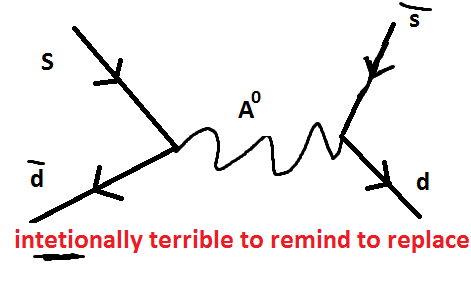
\includegraphics[scale=0.5]{figs/kill_me.png}
\end{center}
\caption{\textit{Feynman Diagram for Kaon mixing in aspon theory }}
\label{asponkaon}
\end{figure}


Generalisations of the aspon model are easy to construct and are the de-facto presentation in \cite{SCPV5}. It is possible to understand what was meant by SCPV being more ``natural" than XCPV in \cite{SCPV1}, simply by thinking that the symmetry breaking mechanism of the Higgs is more natural than the CKM matrix. 


These generalisations simply rely on creating new fields and observing whether or not they have non-removable complex phases in VEVs and their physical effect after symmetry breaking. To be totally general the symmetry breaking need not be Higgs, but for all intents and purposes it usually will be.

In these generalised theories, the particles generated are called ``spurions" of which the $\chi^\alpha$ Higgs particles are specific examples of. SCPV is always related to symmetry breaking of the $\mathrm{U}(1)$ lie group, otherwise, despite VEV having complex phase, it will not show physically. Another important point is the requirement for at least two spurions, for even if there were a non-removable vacuum value like
\begin{align*}
\braket{0|\hat{G}_{CP}|0} = r e^{i\theta}
\end{align*}
As there is only one, this phase will never turn up measurably, one requires a phase difference (just as in QM) for it to be physical.

\subsection{SCPV. Conclusion}
Despite in general having quite an abstract formulation, SCPV is quite an interesting competitor for explaining CPV. Unfortunately, the mathematical details remain beyond the comprehension of the writer's current abilities. Hence, interesting ideas like exactly how new states are predicted have not been attempted. Still, seeing how complex ideas in particle physical physics can be represented by simple symmetry conditions, just as complex ideas can be represented by Feynman diagrams, makes it a far more approachable subject for an undergraduate.

As what has been discussed is such a general condition it is quite robust to how long it may remain experimentally unfalsifiable. This is not an attractive quality. One condition for falsification would be if XCPV is found to be necessary, as that would contradict the result of part D. What are perhaps more interesting are explicit SCPV theories which make falsifiable predictions. For example the aspon model makes the prediction that for $K^0$ mixing the CP parameters must $Re(\frac{\epsilon'}{\epsilon}) \leq 10^{-5}$ \cite{SCPV7}. Comparing this to the experimental result given in the Neutral Kaon Mixing section, $Re(\frac{\epsilon'}{\epsilon})=0.00166 \pm 0.00023$ it is seen that the aspon method \textit{has} been falsified. 

Quite a few modern theories are difficult if nigh on impossible to falsify. It is refreshing to have dealt with an idea that has been proven wrong. Still, SCPV remains in many other prominent models. Aspon theory is introduced purely as an explanatory example.





\end{document}